The Volume/Balance module (\verb=Vol_Bal=) acts as the hub for processing incoming digital audio signals, forwarded from WM8731 via the \verb=Snd_Driver= module. As such, \verb=Vol_Bal= also keeps internal registers in the module \verb=Current_Vol_Bal= that holds volume (4-bit unsigned) and balance levels (4-bit signed), as well as a mute signal (std\_logic). These registers update via the one-hot coded input signal \verb=kb_input= applied by the \verb=Keyboard= module. Consequently, the values they hold are not only used as signals (\verb=i_volume_lvl=, \verb=i_balance_lvl=, \verb=i_mute=) for the internal submodule that process the \verb=LADC= and \verb=RADC= inputs, but also as module outputs connected to the \verb=VGA_Driver= so that they can be rendered on the screen.

\begin{figure}[h]
  \centering
  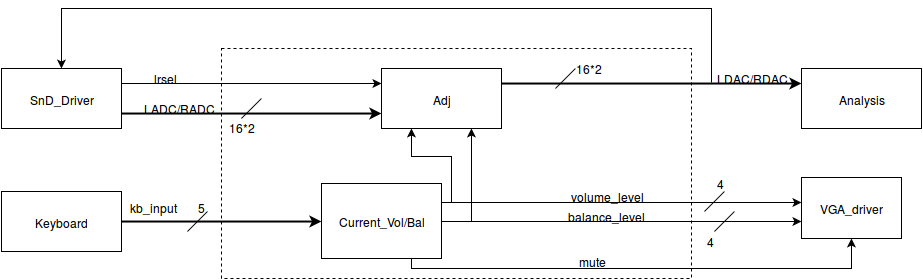
\includegraphics[width=16cm]{volbal}
  \caption{An overview of the Vol\_Bal module's internal workings.}
  \label{fig:vol_bal}
\end{figure}

The main function of the Volume/Balance module is to make requested adjustments to incoming values \verb=LADC= and \verb=RADC=, which represent measured amplitudes of the sound signal at distinct times. The sound will be adjusted for volume and balance by the functions:

\verb=   =$$A_{l\_new} = A_{l\_old} \cdot (1/\sqrt{2})^{n + m}\qquad\ ,\ m = 0\ for\ m < 0$$
\verb=   =$$A_{r\_new} = A_{r\_old} \cdot (1/\sqrt{2})^{n + |m|}\qquad,\ m = 0\ for\ m > 0\ ,$$

where $A$ is the amplitude, $n$ the volume level and $m$ the balance. \verb=lrsel= is used as a control signal for selecting the channel and the correct function. Resulting outputs \verb=LDAC= and \verb=RDAC= are forwarded to \verb=Snd_Driver= and to one instance of the \verb=Analysis= modules.

Ultimately, the user have the ability to digitally adjust the input sound by decreasing the volume in 3 dB decrements, down to -30 dB, and additionally regulate balance bias by further reducing volume by up to another 15 dB on a single left/right audio channel. There is also a mute function which is conveyed by \verb=kb_input=. When active, the register driving the \verb=mute= signal essentially blanks any $A_{new}$ values on the \verb=LDAC/RDAC= outputs.


